\documentclass{article}

\usepackage{array,calc} 
\usepackage{graphics}
\usepackage{amsmath}
%\usepackage{indentfirst}
\usepackage[utf8]{inputenc}
\usepackage{url}
\usepackage{fullpage}

\newcommand{\ba}{ {\boldsymbol a} }
\newcommand{\bA}{ {\boldsymbol A} }
\newcommand{\bb}{ {\boldsymbol b} }
\newcommand{\bB}{ {\boldsymbol B} }
\newcommand{\bc}{ {\boldsymbol c} }
\newcommand{\bC}{ {\boldsymbol C} }
\newcommand{\bd}{ {\boldsymbol d} }
\newcommand{\bD}{ {\boldsymbol D} }
\newcommand{\be}{ {\boldsymbol e} }
\newcommand{\bE}{ {\boldsymbol E} }
\newcommand{\boldf}{ {\boldsymbol f} }
\newcommand{\bF}{ {\boldsymbol F} }
\newcommand{\bg}{ {\boldsymbol g} }
\newcommand{\bG}{ {\boldsymbol G} }
\newcommand{\bh}{ {\boldsymbol h} }
\newcommand{\bH}{ {\boldsymbol H} }
\newcommand{\bi}{ {\boldsymbol i} }
\newcommand{\bI}{ {\boldsymbol I} }
\newcommand{\bj}{ {\boldsymbol j} }
\newcommand{\bJ}{ {\boldsymbol J} }
\newcommand{\bk}{ {\boldsymbol k} }
\newcommand{\bK}{ {\boldsymbol K} }
\newcommand{\bl}{ {\boldsymbol l} }
\newcommand{\bL}{ {\boldsymbol L} }
\newcommand{\bm}{ {\boldsymbol m} }
\newcommand{\bM}{ {\boldsymbol M} }
\newcommand{\bn}{ {\boldsymbol n} }
\newcommand{\bN}{ {\boldsymbol N} }
\newcommand{\bo}{ {\boldsymbol o} }
\newcommand{\bO}{ {\boldsymbol O} }
\newcommand{\bp}{ {\boldsymbol p} }
\newcommand{\bP}{ {\boldsymbol P} }
\newcommand{\bq}{ {\boldsymbol q} }
\newcommand{\bQ}{ {\boldsymbol Q} }
\newcommand{\br}{ {\boldsymbol r} }
\newcommand{\bR}{ {\boldsymbol R} }
\newcommand{\bs}{ {\boldsymbol s} }
\newcommand{\bS}{ {\boldsymbol S} }
\newcommand{\bt}{ {\boldsymbol t} }
\newcommand{\bT}{ {\boldsymbol T} }
\newcommand{\bu}{ {\boldsymbol u} }
\newcommand{\bU}{ {\boldsymbol U} }
\newcommand{\bv}{ {\boldsymbol v} }
\newcommand{\bV}{ {\boldsymbol V} }
\newcommand{\bw}{ {\boldsymbol w} }
\newcommand{\bW}{ {\boldsymbol W} }
\newcommand{\bx}{ {\boldsymbol x} }
\newcommand{\bX}{ {\boldsymbol X} }
\newcommand{\by}{ {\boldsymbol y} }
\newcommand{\bY}{ {\boldsymbol Y} }
\newcommand{\bz}{ {\boldsymbol z} }
\newcommand{\bZ}{ {\boldsymbol Z} }


\newcommand{\balph}{ {\boldsymbol \alpha} }
\newcommand{\balpha}{ {\boldsymbol \alpha} }
\newcommand{\bbet}{ {\boldsymbol \beta} }
\newcommand{\bbeta}{ {\boldsymbol \beta} }
\newcommand{\bgam}{ {\boldsymbol \gamma} }
\newcommand{\bgamma}{ {\boldsymbol \gamma} }
\newcommand{\bGamma}{ {\boldsymbol \Gamma} }
\newcommand{\bdelta}{ {\boldsymbol \delta} }
\newcommand{\bDelta}{ {\boldsymbol \Delta} }
\newcommand{\beps}{ {\boldsymbol \epsilon} }
\newcommand{\bepsilon}{ {\boldsymbol \epsilon} }
\newcommand{\bphi}{ {\boldsymbol \phi} }
\newcommand{\bPhi}{ {\boldsymbol \Phi} }
\newcommand{\bpi}{ {\boldsymbol \pi} }
\newcommand{\bkap}{ {\boldsymbol \kappa} }
\newcommand{\bkappa}{ {\boldsymbol \kappa} }
\newcommand{\bKappa}{ {\boldsymbol \Kappa} }
\newcommand{\blam}{ {\boldsymbol \lambda} }
\newcommand{\blambda}{ {\boldsymbol \lambda} }
\newcommand{\bLambda}{ {\boldsymbol \Lambda} }
\newcommand{\bmu}{ {\boldsymbol \mu} }
\newcommand{\bMu}{ {\boldsymbol \Mu} }
\newcommand{\bet}{ {\boldsymbol \eta} }
\newcommand{\bome}{ {\boldsymbol \omega} }
\newcommand{\bomega}{ {\boldsymbol \omega} }
\newcommand{\bOmega}{ {\boldsymbol \Omega} }
\newcommand{\bnabla}{ {\boldsymbol \nabla} }
\newcommand{\brho}{ {\boldsymbol \rho} }
\newcommand{\bsigma}{ {\boldsymbol \sigma} }
\newcommand{\bSig}{ {\boldsymbol \Sigma} }
\newcommand{\bSigma}{ {\boldsymbol \Sigma} }
\newcommand{\btau}{ {\boldsymbol \tau} }
\newcommand{\btheta}{ {\boldsymbol \theta} }
\newcommand{\bTheta}{ {\boldsymbol \Theta} }
\newcommand{\bzeta}{ {\boldsymbol \zeta} }
\newcommand{\bPsi}{ {\boldsymbol \Psi} }

\newcommand{\bzero}{ {\boldsymbol 0} }
\newcommand{\bones}{ {\boldsymbol 1} }

\newcommand{\given}{\,|\,}

\newcommand{\vs}{{\cal V}}
\newcommand{\sS}{{\cal S}}
\newcommand{\Ss}{{\cal S}}
\newcommand{\Field}{{\cal F}}
\newcommand{\colsp}{{\cal C}}
\newcommand{\nullsp}{{\cal N}}
\newcommand{\rowsp}{{\cal R}}

\newcommand{\tildeC}{\tilde{C}}
\newcommand{\tildeK}{\tilde{K}}
\newcommand{\tildew}{\tilde{w}}
\newcommand{\tildebw}{\tilde{\bw}}
\newcommand{\tildebW}{\tilde{\bW}}
\newcommand{\calC}{{\cal C}}
\newcommand{\calcbC}{{\bf {\cal C}}}
\newcommand{\calS}{{\cal S}}
\newcommand{\calcbS}{{\bf {\cal S}}}

\newcommand{\np}{\newpage}

\newcommand{\mywid}{2.1in}
\newcommand{\mywidr}{2.2in}
\newcommand{\myht}{1.5in}
\newcommand{\myhts}{1.1in}
\newcommand{\myupvspace}{-\myht}
\newcommand{\myupvspaces}{-\myhts}
\newcommand{\mydnvspace}{.3in}
\newcommand{\myhspace}{2.2in}
\newcommand{\myhmidspace}{1.1in}
\newcommand{\mybotvspace}{.1in}
\newcommand{\vsp}{\vspace{2ex}}

\newcommand{\proglang}[1]{{\textsf{#1}}}
\newcommand{\R}{\proglang{R}}
\newcommand{\pkg}[1]{{\normalfont\fontseries{b}\selectfont #1}}
\newcommand{\pbs}[1]{\let\tmp\\#1\let\\\tmp} 


 


\usepackage{Sweave}
\begin{document}


\title{Bayesian Dynamic Modeling for Space-time Data in \proglang{R}}

\author{Andrew O. Finley}
\maketitle

%\section{Data preparation and initial exploration}

We make use of several libraries in the following example session, including:

\begin{tabular}{*2{>{\pbs{\raggedright}}p{\columnwidth/2 -3\tabcolsep}}}
  \begin{itemize}\setlength{\itemsep}{-0.05cm}
  \item \verb@library(fields)@
  \item \verb@library(geoR)@
  \item \verb@library(MBA)@
  \item \verb@library(spBayes)@
  %%\item \verb@library(raster)@
  \end{itemize}
  &
  %% \begin{itemize}\setlength{\itemsep}{-0.05cm}
  %% %%\item \verb@library(rgdal)@
  %% %%\item \verb@library(RgoogleMaps)@
  %% %%\item \verb@library(spBayes)@
  %% %%\item \verb@library(yaImpute)@
  %% \end{itemize}
\end{tabular} 

There are many different kinds of spatio-temporal data and extensive statistical literature that addresses most common settings. The approach adopted here applies to the setting where space is viewed as continuous, but time is taken to be discrete. Put another way, we view the data as a time series of spatial process realizations and work in the setting of dynamic models. Building upon previous work in the setting of dynamic models by West and Harrison (1997), several authors, including Tonellato (1997), Stroud et al. (2001) and Gelfand et al. (2005), proposed dynamic frameworks to model residual spatial and temporal dependence. These proposed frameworks are flexible and easily extended to accommodate nonstationary and multivariate outcomes.

\section{Dynamic spatio-temporal models}\label{models}
Dynamic linear models, or state-space models, have gained tremendous
popularity in recent years in fields as disparate as engineering, economics, genetics, and ecology. They offer a versatile framework for fitting several time-varying models (West and Harrison 1997).  Gelfand et al. (2005) adapted the dynamic modeling framework to spatio-temporal models with spatially varying coefficients. Alternative adaptations of dynamic linear models to space-time data can be found in Stroud et al. (2001) and Tonellato (1997). 

Here we consider a fairly basic, yet flexible, formulation. Suppose, $y_t(\bs)$ denotes the observation at location $\bs$ and time
$t$. We model $y_t(\bs)$ through a \emph{measurement equation} that
provides a regression specification with a space-time varying
intercept and  serially and spatially
uncorrelated zero-centered Gaussian disturbances as measurement error
$\epsilon_t(\bs)$. Next a \emph{transition equation} introduces a $p
\times 1$ coefficient vector, say $\bbeta_t$, which is a purely
temporal component (i.e., time-varying regression parameters), and a
spatio-temporal component $u_t(\bs)$. Both these are generated through
transition equations, capturing their Markovian dependence in
time. While the transition equation of the purely temporal component
is akin to usual state-space modeling, the spatio-temporal component is
generated using Gaussian spatial processes. The overall model is written as
\begin{align}\label{Eq: Dynamic_ST_Model}
y_t(\bs) & = \bx_t(\bs)'\bbeta_t + u_t(\bs) + \epsilon_t(\bs),\quad \epsilon_t(\bs)\stackrel{ind.}\sim N(0,\tau_{t}^2)\; ;\nonumber \\
\bbeta_t & = \bbeta_{t-1} + \bet_t,\quad \bet_t\stackrel{i.i.d.}\sim
N(0,\bSigma_{\eta})\; ;\nonumber \\
u_t(\bs) &= u_{t-1}(\bs) + w_t(\bs),\quad w_t(\bs) \stackrel{ind.}{\sim} GP\left(\bzero, C_t(\cdot,\btheta_t)\right),\quad t=1,2,\ldots,N_t\;,
\end{align}
where the abbreviations $ind.$ and $i.i.d$ are \emph{independent} and \emph{independent and identically distributed}, respectively. Here $\bx_t(\bs)$ is a $p\times 1$ vector of predictors and $\bbeta_t$ is a $p\times 1$ vector of coefficients. In addition to an intercept, $\bx_t(\bs)$ can include location specific variables useful for explaining the variability in $y_t(\bs)$. The $GP(\bzero, C_t(\cdot,\btheta_t))$ denotes a spatial Gaussian process (a Gaussian process defined over an Euclidean spatial domain; see, e.g., Cressie 1993) with covariance function $C_{t}(\cdot;\btheta_t)$. We customarily specify $C_{t}(\bs_1,\bs_2;\btheta_t)=\sigma_t^2\rho(\bs_1,\bs_2;\phi_t)$, where $\btheta_t = \{\sigma_t^2,\phi_t\}$ and $\rho(\cdot;\phi)$ is a \emph{correlation function} with $\phi$ controlling the correlation decay and $\sigma_t^2$ represents the spatial variance component. An exponential function is often used to define the spatial correlation structure, e.g., $C_{t}(\bs_1,\bs_2;\btheta_t)=\sigma_t^2\exp(-\phi_t\|\bs_1-\bs_2\|)$, where $\|\bs_1-\bs_2\|$ is the Euclidean distance between the sites $\bs_1$ and $\bs_2$. However, any \emph{valid} spatial correlation function could be used, see, e.g., Cressie 1993, Chil\'{e}s and Delfiner 1999, and Banerjee et al. 2004. We further assume $\bbeta_0 \sim N(\bm_0, \bSigma_0)$ and $u_0(\bs) \equiv 0$, which completes the prior specifications leading to a well-identified Bayesian hierarchical model and also yield reasonable dependence structures. In practice, estimation of model parameters are usually very robust to these hyper-prior specifications. Also note that (\ref{Eq: Dynamic_ST_Model}) reduces to a simple spatial regression model for $t=1$.  

We consider settings where the inferential interest lies in spatial prediction or interpolation over a region for a set of discrete time points. We also assume that the same locations are monitored for each time point resulting in a space-time matrix whose rows index the locations and columns index the time points, i.e. the $(i,j)$-th element is $y_j(\bs_i)$. Our algorithm will accommodate the situation where some cells of the space-time data matrix may have missing observations, as is common in monitoring environmental variables.

\section{Data and computing}\label{data}
For this illustrative analysis, we consider monthly temperature data observed on a network of weather stations between January 2000 and December 2002. For brevity we only consider stations over a portion of New England. We also have elevation in meters for each station, which will serve as a covariate in the subsequent analysis. In the code below, \verb@N.t@ is the number of months and \verb@n@ is the number of observations per month. 

\begin{Schunk}
\begin{Sinput}
> set.seed(1)
> data("NETemp.dat")
> ne.temp <- NETemp.dat
> ne.temp <- ne.temp[ne.temp[, "UTMX"] > 5500000 & ne.temp[, "UTMY"] > 
+     3e+06, ]
> y.t <- ne.temp[, 4:27]
> N.t <- ncol(y.t)
> n <- nrow(y.t)
\end{Sinput}
\end{Schunk}

Here we set some observations to \verb@NA@ to illustrate the predictive ability of this modeling framework. The true values of the holdout observations are retained for subsequent comparison.

\begin{Schunk}
\begin{Sinput}
> miss <- sample(1:N.t, 10)
> holdout.station.id <- 5
> y.t.holdout <- y.t[holdout.station.id, miss]
> y.t[holdout.station.id, miss] <- NA
> coords <- as.matrix(ne.temp[, c("UTMX", "UTMY")]/1000)
> max.d <- max(iDist(coords))
> plot(coords, xlab = "Easting (km)", ylab = "Northin (km)")
\end{Sinput}
\end{Schunk}
\clearpage
\begin{figure}
\begin{center}
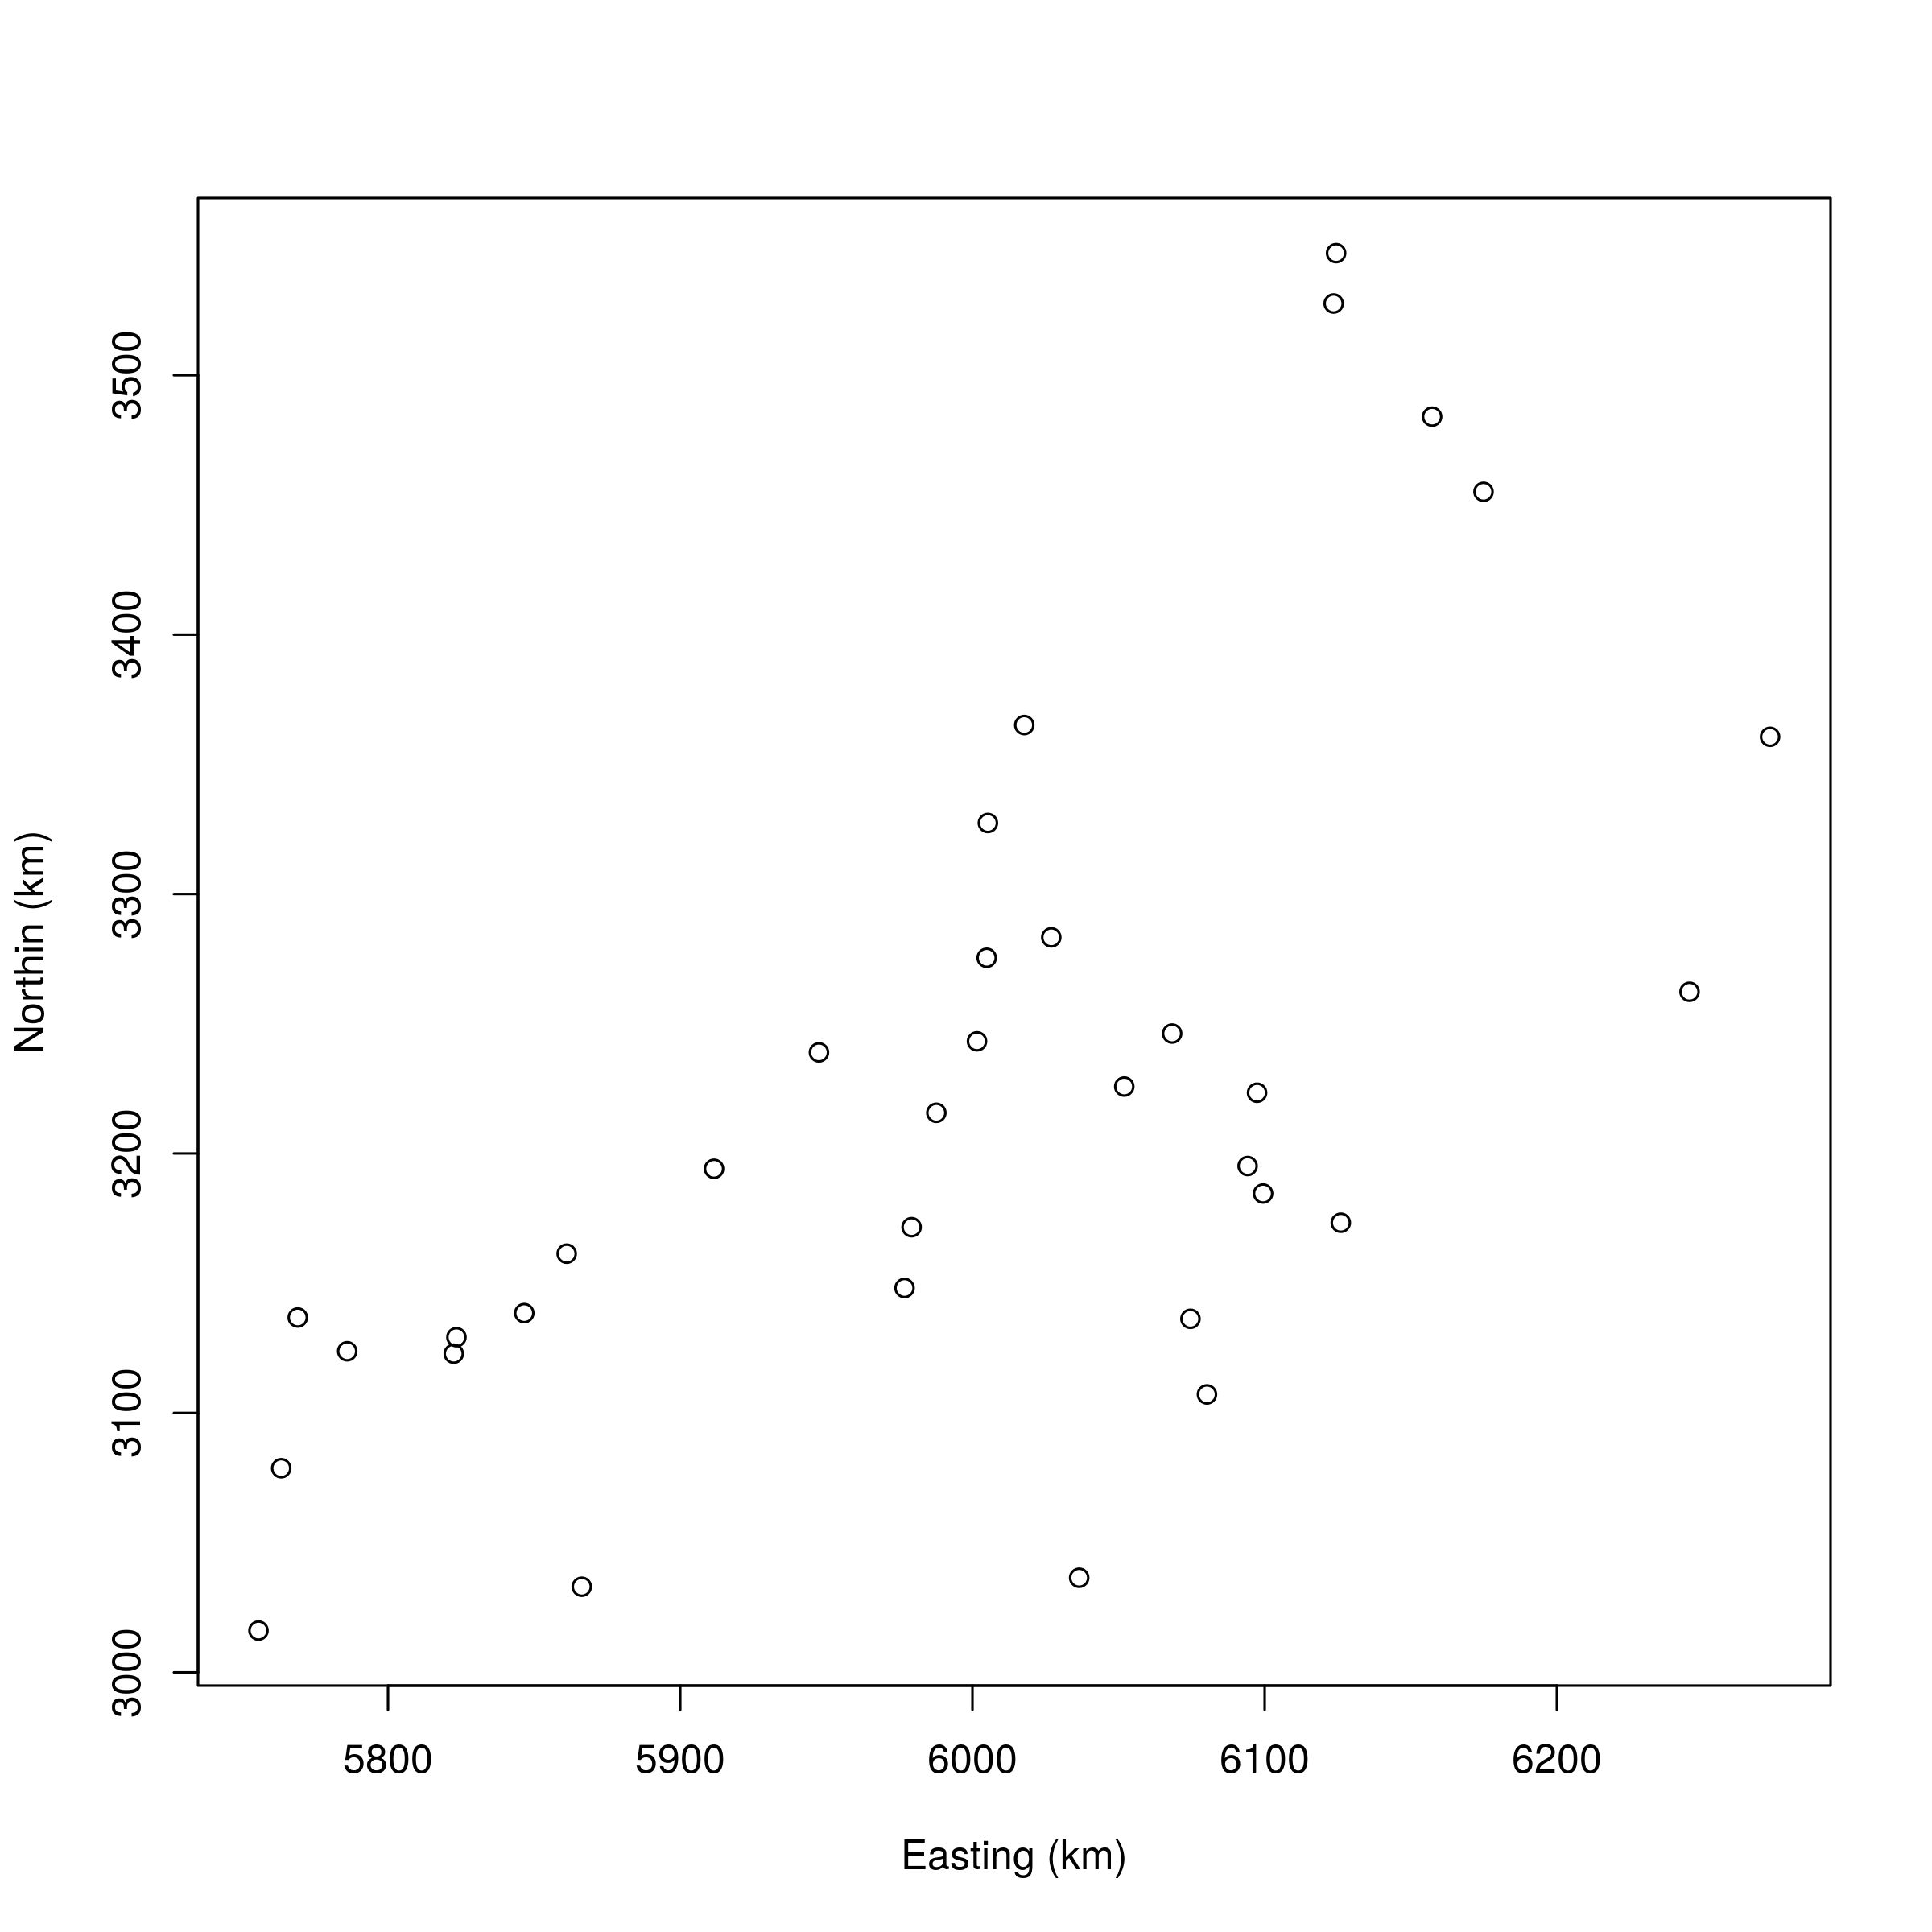
\includegraphics[width=10cm]{figures/fig-data}
\end{center}
\caption{Weather station locations.}
\label{fig:fig-data}
\end{figure}

Next we need to specify priors for the numerous parameters. A variogram analysis for each time step is useful for guiding prior and hyperparameter specification. In the code below, \verb@p@ is the number of regression coefficients, i.e., corresponding to the intercept and elevation.

\begin{Schunk}
\begin{Sinput}
> p <- 2
> starting <- list(beta = rep(0, N.t * p), phi = rep(3/(0.5 * max.d), 
+     N.t), sigma.sq = rep(2, N.t), tau.sq = rep(1, N.t), sigma.eta = diag(rep(0.01, 
+     p)))
> tuning <- list(phi = rep(0.75, N.t))
> priors <- list(beta.0.Norm = list(rep(0, p), diag(1000, p)), phi.Unif = list(rep(3/(0.9 * 
+     max.d), N.t), rep(3/(0.05 * max.d), N.t)), sigma.sq.IG = list(rep(2, 
+     N.t), rep(10, N.t)), tau.sq.IG = list(rep(2, N.t), rep(5, N.t)), 
+     sigma.eta.IW = list(2, diag(0.001, p)))
\end{Sinput}
\end{Schunk}

Like \verb@spMvLM@, \verb@spDynLM@ will take a list of symbolic model formula. However, unlike \verb@spMvLM@, each time step must have the same covariates, although their values can change over time.
\begin{Schunk}
\begin{Sinput}
> mods <- lapply(paste(colnames(y.t), "elev", sep = "~"), as.formula)
> n.samples <- 4000
> m.1 <- spDynLM(mods, data = cbind(y.t, ne.temp[, "elev", drop = FALSE]), 
+     coords = coords, starting = starting, tuning = tuning, priors = priors, 
+     get.fitted = TRUE, cov.model = "exponential", n.samples = n.samples, 
+     n.report = 1000)
\end{Sinput}
\begin{Soutput}
----------------------------------------
	General model description
----------------------------------------
Model fit with 34 observations in 24 time steps.

Number of missing observations 10.

Number of covariates 2 (including intercept if specified).

Using the exponential spatial correlation model.

Number of MCMC samples 4000.

Priors and hyperpriors:
	beta normal:
	m_0:	0.000	0.000	
	Sigma_0:
	1000.000	0.000	
	0.000	1000.000	

	sigma.sq_t=1 IG hyperpriors shape=2.00000 and scale=10.00000
	tau.sq_t=1 IG hyperpriors shape=2.00000 and scale=5.00000
	phi_t=1 Unif hyperpriors a=0.00516 and b=0.09281
	---
	sigma.sq_t=2 IG hyperpriors shape=2.00000 and scale=10.00000
	tau.sq_t=2 IG hyperpriors shape=2.00000 and scale=5.00000
	phi_t=2 Unif hyperpriors a=0.00516 and b=0.09281
	---
	sigma.sq_t=3 IG hyperpriors shape=2.00000 and scale=10.00000
	tau.sq_t=3 IG hyperpriors shape=2.00000 and scale=5.00000
	phi_t=3 Unif hyperpriors a=0.00516 and b=0.09281
	---
	sigma.sq_t=4 IG hyperpriors shape=2.00000 and scale=10.00000
	tau.sq_t=4 IG hyperpriors shape=2.00000 and scale=5.00000
	phi_t=4 Unif hyperpriors a=0.00516 and b=0.09281
	---
	sigma.sq_t=5 IG hyperpriors shape=2.00000 and scale=10.00000
	tau.sq_t=5 IG hyperpriors shape=2.00000 and scale=5.00000
	phi_t=5 Unif hyperpriors a=0.00516 and b=0.09281
	---
	sigma.sq_t=6 IG hyperpriors shape=2.00000 and scale=10.00000
	tau.sq_t=6 IG hyperpriors shape=2.00000 and scale=5.00000
	phi_t=6 Unif hyperpriors a=0.00516 and b=0.09281
	---
	sigma.sq_t=7 IG hyperpriors shape=2.00000 and scale=10.00000
	tau.sq_t=7 IG hyperpriors shape=2.00000 and scale=5.00000
	phi_t=7 Unif hyperpriors a=0.00516 and b=0.09281
	---
	sigma.sq_t=8 IG hyperpriors shape=2.00000 and scale=10.00000
	tau.sq_t=8 IG hyperpriors shape=2.00000 and scale=5.00000
	phi_t=8 Unif hyperpriors a=0.00516 and b=0.09281
	---
	sigma.sq_t=9 IG hyperpriors shape=2.00000 and scale=10.00000
	tau.sq_t=9 IG hyperpriors shape=2.00000 and scale=5.00000
	phi_t=9 Unif hyperpriors a=0.00516 and b=0.09281
	---
	sigma.sq_t=10 IG hyperpriors shape=2.00000 and scale=10.00000
	tau.sq_t=10 IG hyperpriors shape=2.00000 and scale=5.00000
	phi_t=10 Unif hyperpriors a=0.00516 and b=0.09281
	---
	sigma.sq_t=11 IG hyperpriors shape=2.00000 and scale=10.00000
	tau.sq_t=11 IG hyperpriors shape=2.00000 and scale=5.00000
	phi_t=11 Unif hyperpriors a=0.00516 and b=0.09281
	---
	sigma.sq_t=12 IG hyperpriors shape=2.00000 and scale=10.00000
	tau.sq_t=12 IG hyperpriors shape=2.00000 and scale=5.00000
	phi_t=12 Unif hyperpriors a=0.00516 and b=0.09281
	---
	sigma.sq_t=13 IG hyperpriors shape=2.00000 and scale=10.00000
	tau.sq_t=13 IG hyperpriors shape=2.00000 and scale=5.00000
	phi_t=13 Unif hyperpriors a=0.00516 and b=0.09281
	---
	sigma.sq_t=14 IG hyperpriors shape=2.00000 and scale=10.00000
	tau.sq_t=14 IG hyperpriors shape=2.00000 and scale=5.00000
	phi_t=14 Unif hyperpriors a=0.00516 and b=0.09281
	---
	sigma.sq_t=15 IG hyperpriors shape=2.00000 and scale=10.00000
	tau.sq_t=15 IG hyperpriors shape=2.00000 and scale=5.00000
	phi_t=15 Unif hyperpriors a=0.00516 and b=0.09281
	---
	sigma.sq_t=16 IG hyperpriors shape=2.00000 and scale=10.00000
	tau.sq_t=16 IG hyperpriors shape=2.00000 and scale=5.00000
	phi_t=16 Unif hyperpriors a=0.00516 and b=0.09281
	---
	sigma.sq_t=17 IG hyperpriors shape=2.00000 and scale=10.00000
	tau.sq_t=17 IG hyperpriors shape=2.00000 and scale=5.00000
	phi_t=17 Unif hyperpriors a=0.00516 and b=0.09281
	---
	sigma.sq_t=18 IG hyperpriors shape=2.00000 and scale=10.00000
	tau.sq_t=18 IG hyperpriors shape=2.00000 and scale=5.00000
	phi_t=18 Unif hyperpriors a=0.00516 and b=0.09281
	---
	sigma.sq_t=19 IG hyperpriors shape=2.00000 and scale=10.00000
	tau.sq_t=19 IG hyperpriors shape=2.00000 and scale=5.00000
	phi_t=19 Unif hyperpriors a=0.00516 and b=0.09281
	---
	sigma.sq_t=20 IG hyperpriors shape=2.00000 and scale=10.00000
	tau.sq_t=20 IG hyperpriors shape=2.00000 and scale=5.00000
	phi_t=20 Unif hyperpriors a=0.00516 and b=0.09281
	---
	sigma.sq_t=21 IG hyperpriors shape=2.00000 and scale=10.00000
	tau.sq_t=21 IG hyperpriors shape=2.00000 and scale=5.00000
	phi_t=21 Unif hyperpriors a=0.00516 and b=0.09281
	---
	sigma.sq_t=22 IG hyperpriors shape=2.00000 and scale=10.00000
	tau.sq_t=22 IG hyperpriors shape=2.00000 and scale=5.00000
	phi_t=22 Unif hyperpriors a=0.00516 and b=0.09281
	---
	sigma.sq_t=23 IG hyperpriors shape=2.00000 and scale=10.00000
	tau.sq_t=23 IG hyperpriors shape=2.00000 and scale=5.00000
	phi_t=23 Unif hyperpriors a=0.00516 and b=0.09281
	---
	sigma.sq_t=24 IG hyperpriors shape=2.00000 and scale=10.00000
	tau.sq_t=24 IG hyperpriors shape=2.00000 and scale=5.00000
	phi_t=24 Unif hyperpriors a=0.00516 and b=0.09281
	---
-------------------------------------------------
		Sampling
-------------------------------------------------
Sampled: 999 of 4000, 24.98%
Report interval Mean Metrop. Acceptance rate: 77.58%
Overall Metrop. Acceptance rate: 77.66%
-------------------------------------------------
Sampled: 1999 of 4000, 49.98%
Report interval Mean Metrop. Acceptance rate: 77.81%
Overall Metrop. Acceptance rate: 77.73%
-------------------------------------------------
Sampled: 2999 of 4000, 74.97%
Report interval Mean Metrop. Acceptance rate: 77.85%
Overall Metrop. Acceptance rate: 77.77%
-------------------------------------------------
Sampled: 3999 of 4000, 99.97%
Report interval Mean Metrop. Acceptance rate: 77.30%
Overall Metrop. Acceptance rate: 77.65%
-------------------------------------------------
\end{Soutput}
\end{Schunk}

\begin{Schunk}
\begin{Sinput}
> burn.in <- floor(0.75 * n.samples)
> quant <- function(x) {
+     quantile(x, prob = c(0.5, 0.025, 0.975))
+ }
> beta <- apply(m.1$p.beta.samples[burn.in:n.samples, ], 2, quant)
> beta.0 <- beta[, grep("Intercept", colnames(beta))]
> beta.1 <- beta[, grep("elev", colnames(beta))]
> par(mfrow = c(2, 1))
> plot(1:N.t, beta.0[1, ], pch = 19, cex = 0.5, xlab = "months", ylab = "beta.0", 
+     ylim = range(beta.0))
> arrows(1:N.t, beta.0[1, ], 1:N.t, beta.0[3, ], length = 0.02, angle = 90)
> arrows(1:N.t, beta.0[1, ], 1:N.t, beta.0[2, ], length = 0.02, angle = 90)
> plot(1:N.t, beta.1[1, ], pch = 19, cex = 0.5, xlab = "months", ylab = "beta.1", 
+     ylim = range(beta.1))
> arrows(1:N.t, beta.1[1, ], 1:N.t, beta.1[3, ], length = 0.02, angle = 90)
> arrows(1:N.t, beta.1[1, ], 1:N.t, beta.1[2, ], length = 0.02, angle = 90)
\end{Sinput}
\end{Schunk}

\begin{figure}
\begin{center}
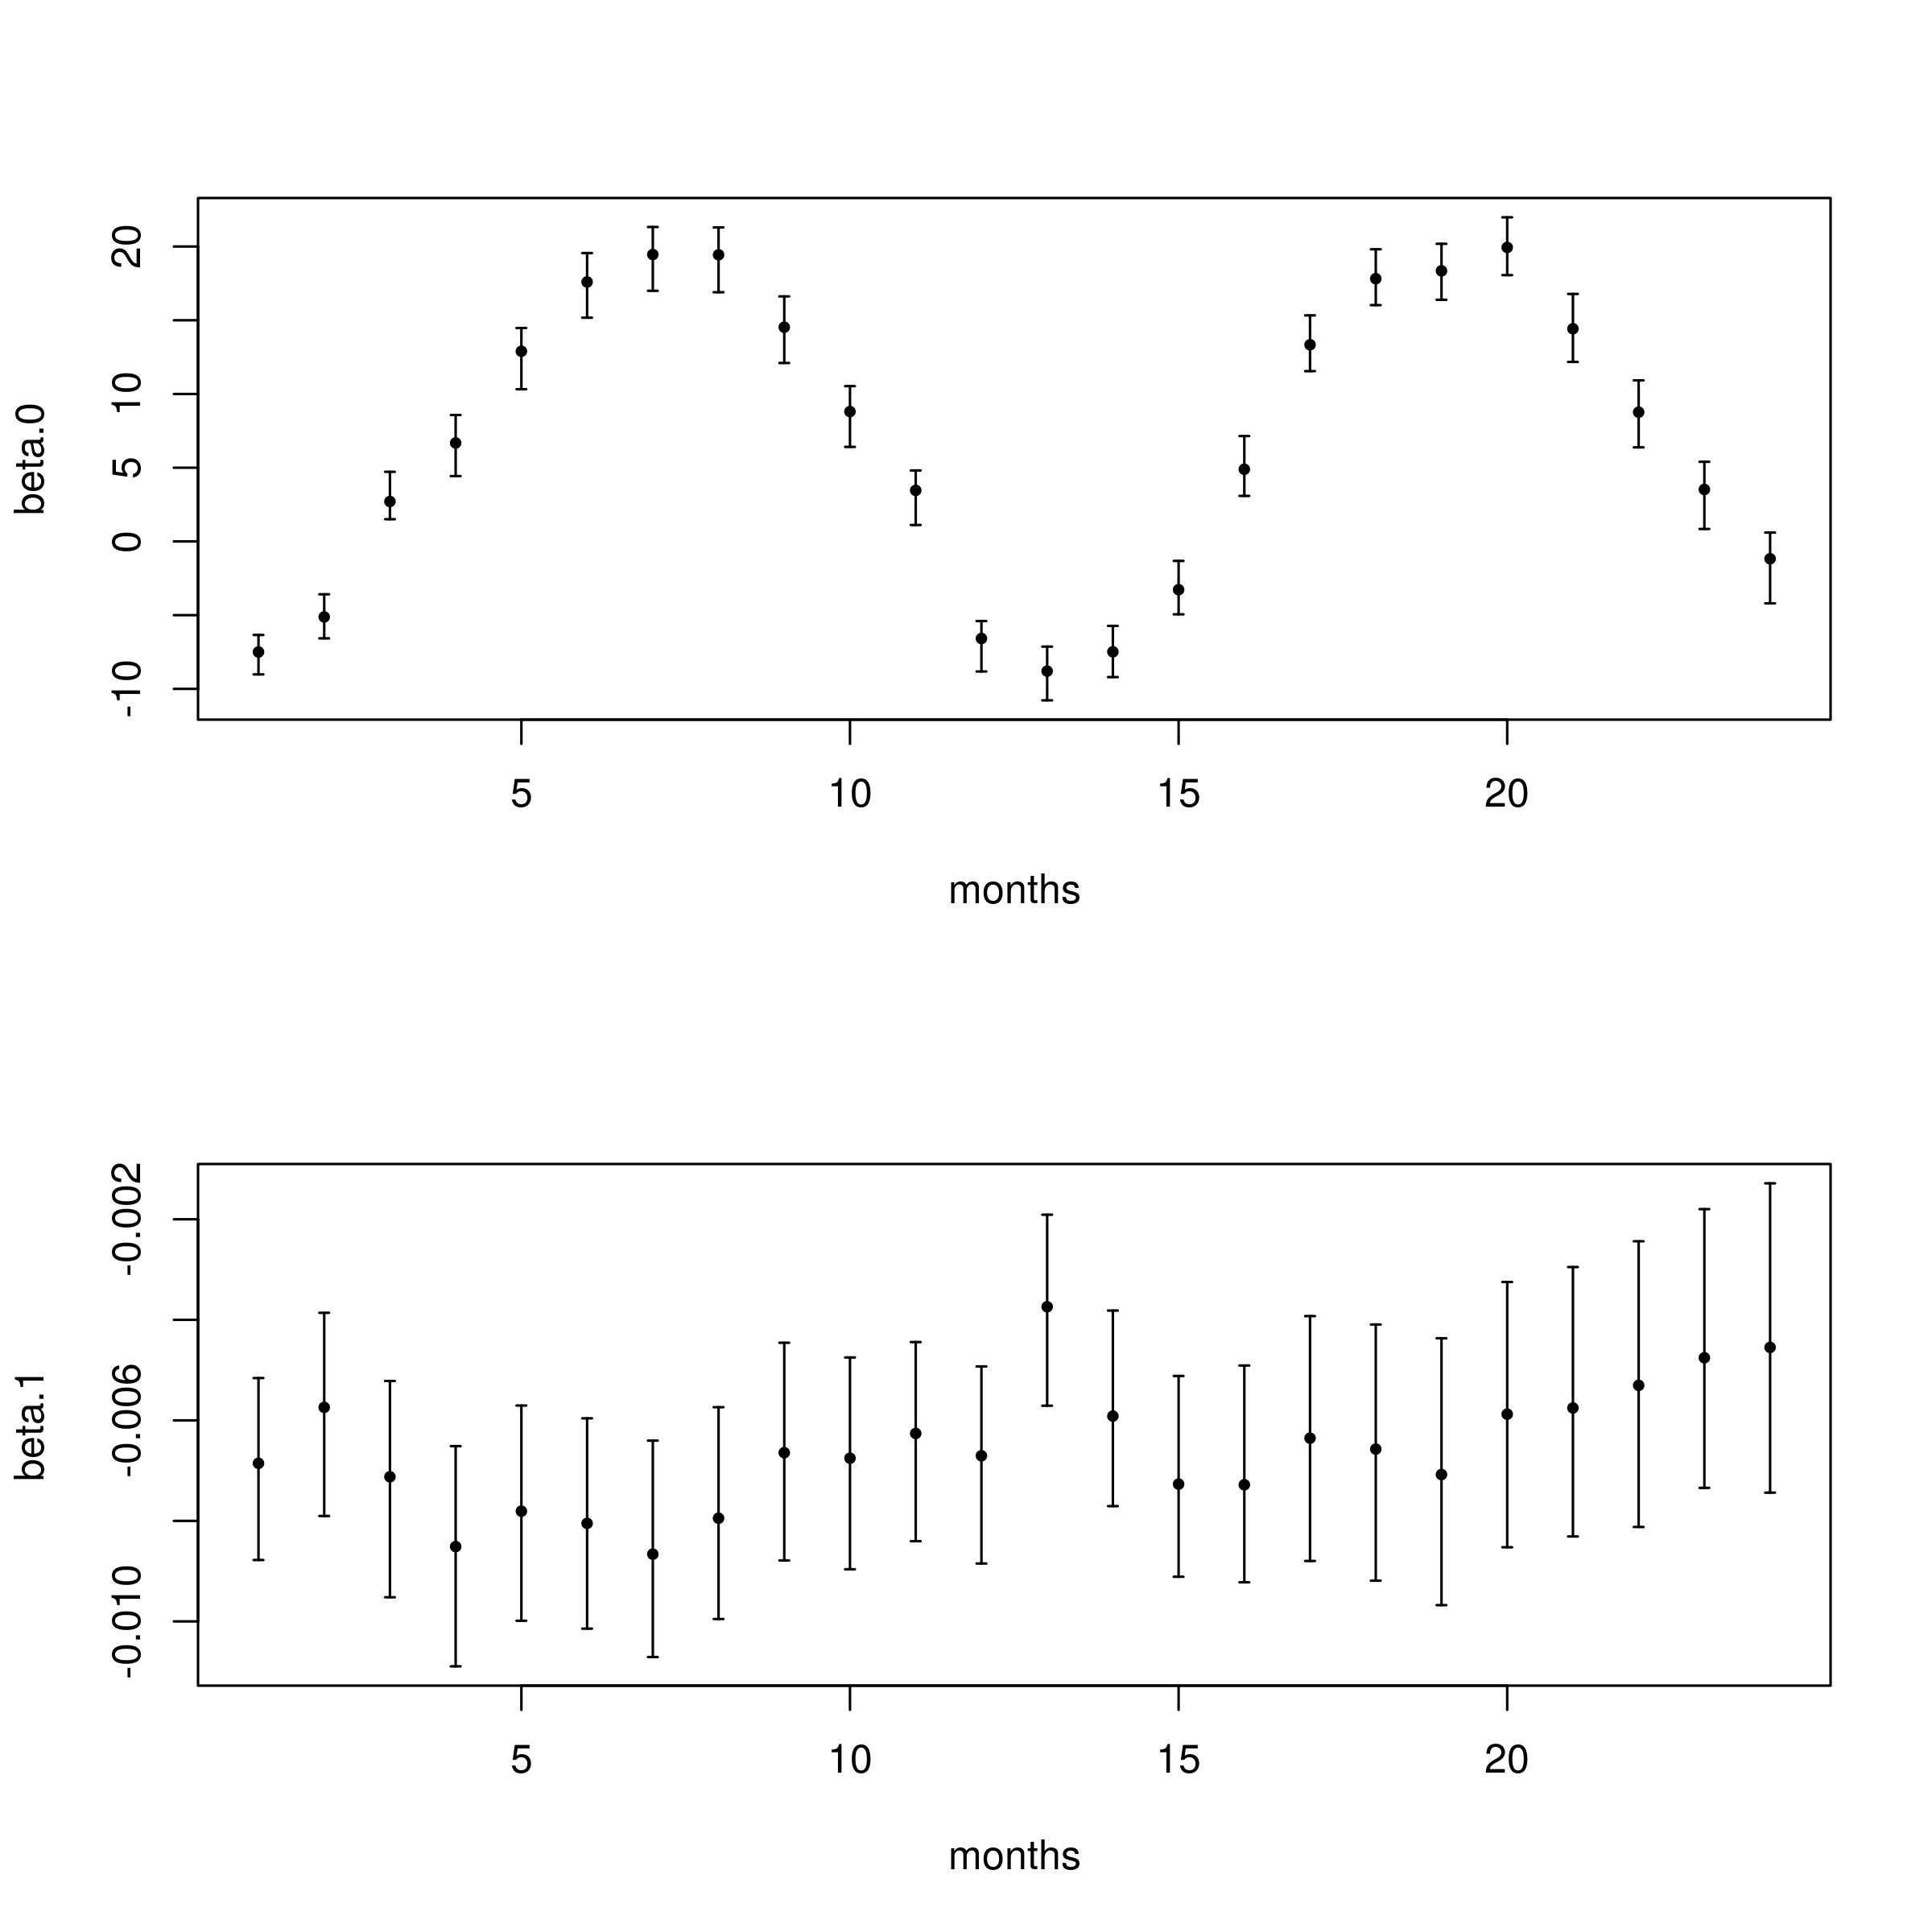
\includegraphics[width=10cm]{figures/fig-beta}
\end{center}
\caption{Evolution of the regression coefficients.}
\label{fig:fig-beta}
\end{figure}

\begin{Schunk}
\begin{Sinput}
> theta <- apply(m.1$p.theta.samples[burn.in:n.samples, ], 2, quant)
> sigma.sq <- theta[, grep("sigma.sq", colnames(theta))]
> tau.sq <- theta[, grep("tau.sq", colnames(theta))]
> phi <- theta[, grep("phi", colnames(theta))]
> par(mfrow = c(3, 1))
> plot(1:N.t, sigma.sq[1, ], pch = 19, cex = 0.5, xlab = "months", 
+     ylab = "sigma.sq", ylim = range(sigma.sq))
> arrows(1:N.t, sigma.sq[1, ], 1:N.t, sigma.sq[3, ], length = 0.02, 
+     angle = 90)
> arrows(1:N.t, sigma.sq[1, ], 1:N.t, sigma.sq[2, ], length = 0.02, 
+     angle = 90)
> plot(1:N.t, tau.sq[1, ], pch = 19, cex = 0.5, xlab = "months", ylab = "tau.sq", 
+     ylim = range(tau.sq))
> arrows(1:N.t, tau.sq[1, ], 1:N.t, tau.sq[3, ], length = 0.02, angle = 90)
> arrows(1:N.t, tau.sq[1, ], 1:N.t, tau.sq[2, ], length = 0.02, angle = 90)
> plot(1:N.t, 3/phi[1, ], pch = 19, cex = 0.5, xlab = "months", ylab = "eff. range (km)", 
+     ylim = range(3/phi))
> arrows(1:N.t, 3/phi[1, ], 1:N.t, 3/phi[3, ], length = 0.02, angle = 90)
> arrows(1:N.t, 3/phi[1, ], 1:N.t, 3/phi[2, ], length = 0.02, angle = 90)
\end{Sinput}
\end{Schunk}

\begin{figure}
\begin{center}
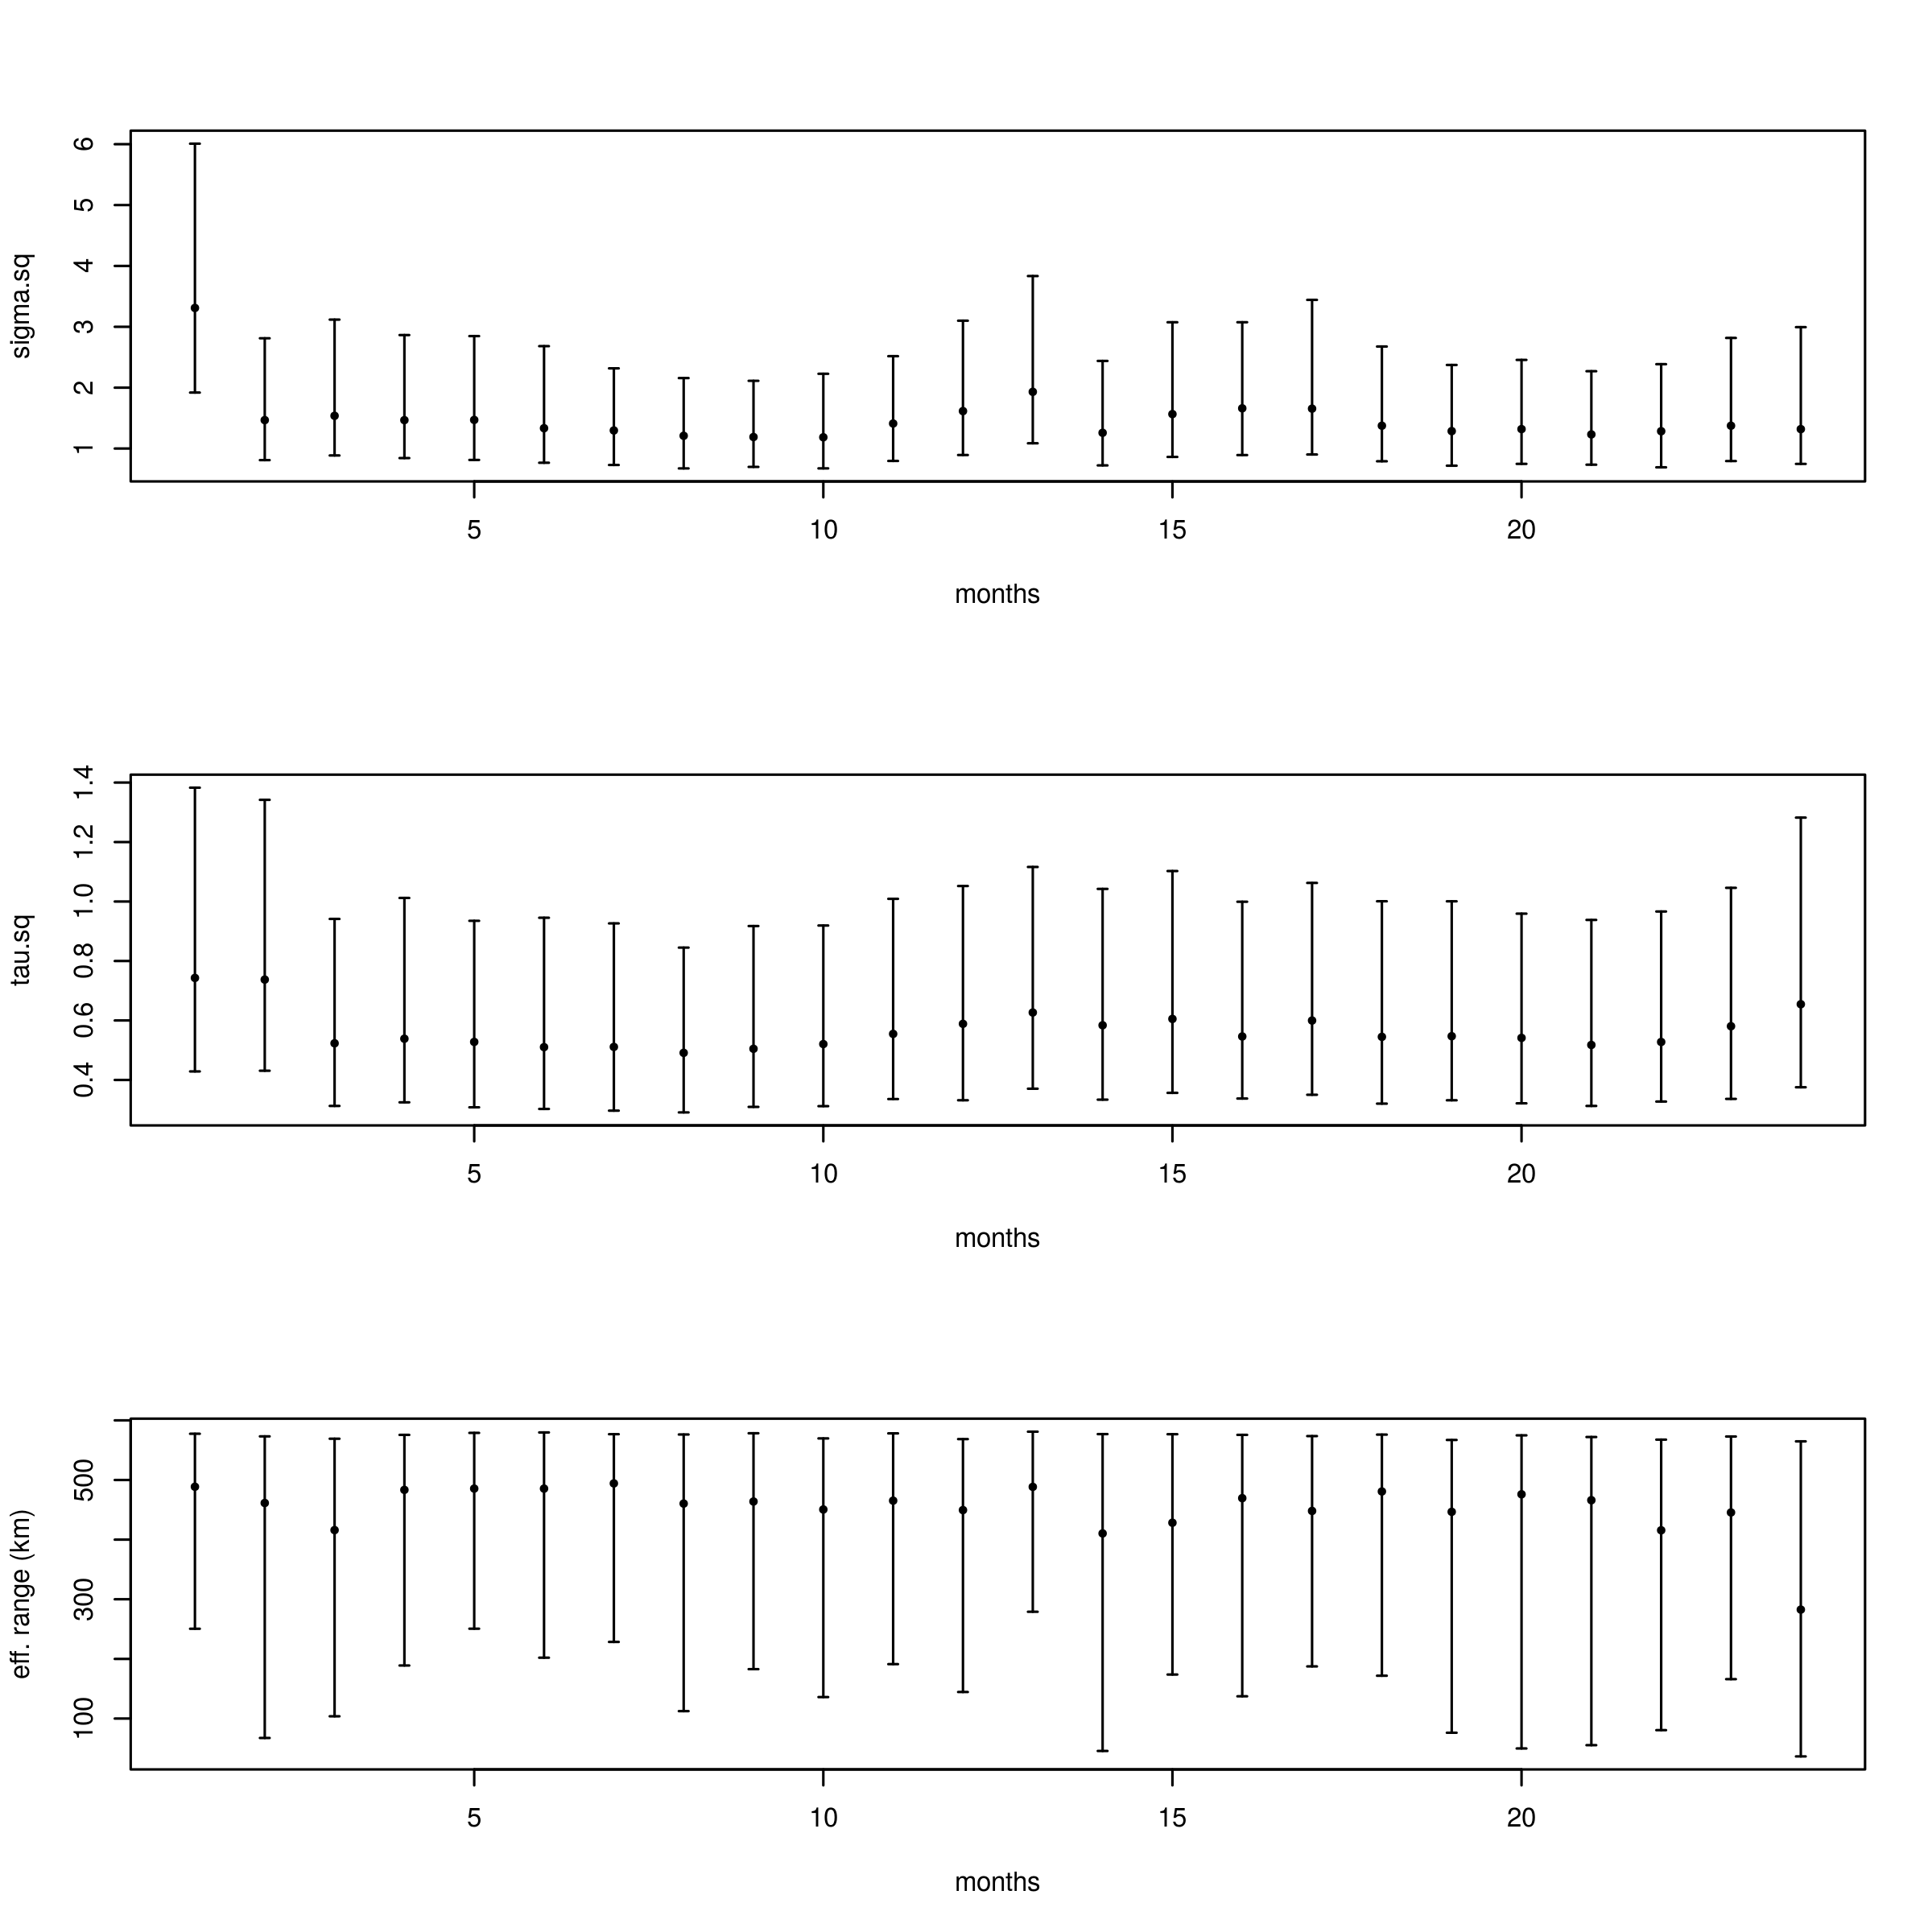
\includegraphics[width=10cm]{figures/fig-theta}
\end{center}
\caption{Evolution of the spatial covariance parameters.}
\label{fig:fig-theta}
\end{figure}

\begin{Schunk}
\begin{Sinput}
> y.hat <- apply(m.1$p.y.samples[, burn.in:n.samples], 1, quant)
> y.hat.med <- matrix(y.hat[1, ], ncol = N.t)
> y.hat.up <- matrix(y.hat[3, ], ncol = N.t)
> y.hat.low <- matrix(y.hat[2, ], ncol = N.t)
> y.obs <- as.vector(as.matrix(y.t[-holdout.station.id, -miss]))
> y.obs.hat.med <- as.vector(y.hat.med[-holdout.station.id, -miss])
> y.obs.hat.up <- as.vector(y.hat.up[-holdout.station.id, -miss])
> y.obs.hat.low <- as.vector(y.hat.low[-holdout.station.id, -miss])
> y.ho <- as.matrix(y.t.holdout)
> y.ho.hat.med <- as.vector(y.hat.med[holdout.station.id, miss])
> y.ho.hat.up <- as.vector(y.hat.up[holdout.station.id, miss])
> y.ho.hat.low <- as.vector(y.hat.low[holdout.station.id, miss])
> par(mfrow = c(1, 2))
> plot(y.obs, y.obs.hat.med, pch = 19, cex = 0.5, xlab = "observed", 
+     ylab = "fitted", main = "Observed vs. fitted")
> arrows(y.obs, y.obs.hat.med, y.obs, y.obs.hat.up, length = 0.02, 
+     angle = 90)
> arrows(y.obs, y.obs.hat.med, y.obs, y.obs.hat.low, length = 0.02, 
+     angle = 90)
> lines(-50:50, -50:50, col = "blue")
> plot(y.ho, y.ho.hat.med, pch = 19, cex = 0.5, xlab = "observed", 
+     ylab = "predicted", , main = "Observed vs. predicted")
> arrows(y.ho, y.ho.hat.med, y.ho, y.ho.hat.up, length = 0.02, angle = 90)
> arrows(y.ho, y.ho.hat.med, y.ho, y.ho.hat.low, length = 0.02, angle = 90)
> lines(-50:50, -50:50, col = "blue")
\end{Sinput}
\end{Schunk}

\begin{figure}
\begin{center}
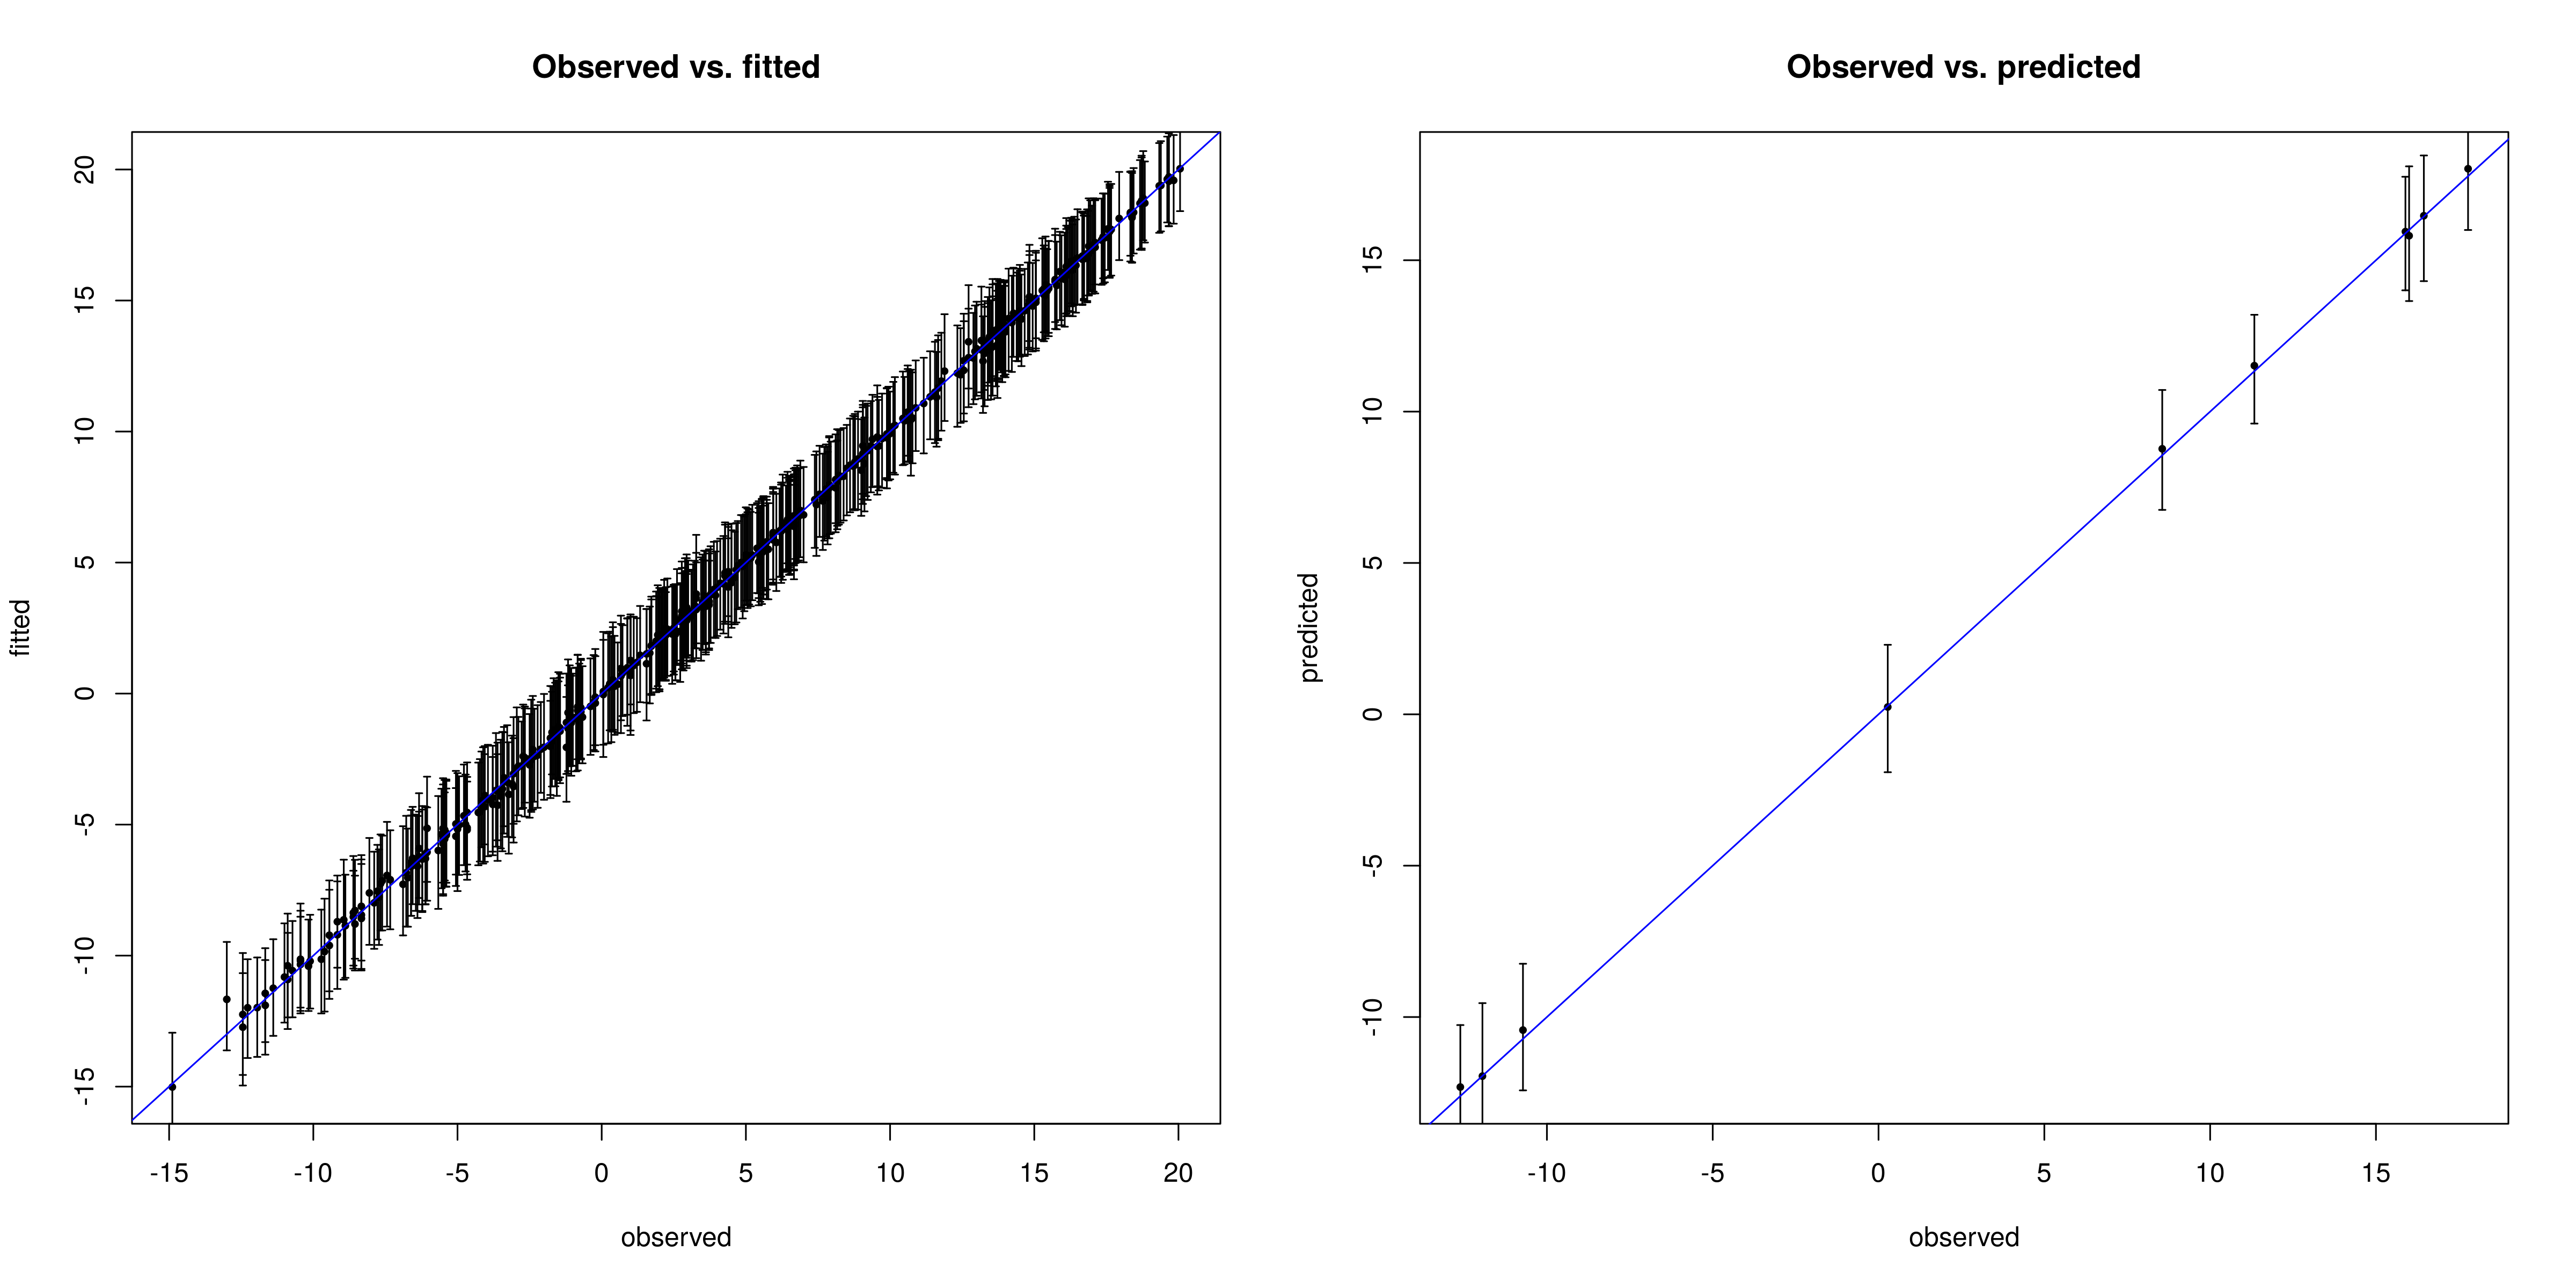
\includegraphics[width=10cm]{figures/fig-pred}
\end{center}
\caption{Fitted values (left) and holdout predicted values (right).}
\label{fig:fig-pred}
\end{figure}

\clearpage

\section{References}

\begin{description}  
\item Banerjee S, Carlin, BP, Gelfand AE (2004) \emph{Hierarchical modeling and analysis for spatial data}. Chapman and Hall/CRC Press, Boca Raton, FL.

\item Chil\'{e}s JP, Delfiner P (1999) \emph{Geostatistics: modelling spatial uncertainty}. Wiley, New York.

\item Cressie NAC (1993) \emph{Statistics for spatial data, 2nd edition}. Wiley, New York.

\item Gelfand AE, Banerjee S, Gamerman D (2005) Univariate and multivariate dynamic spatial modelling. \emph{Environmetrics}, \textbf{16}:465--479

\item Stroud JR, Muller P, Sans\'{o} B (2001) Dynamic models for spatiotemporal data. \emph{Journal of the Royal Statistical Society Series B}, \textbf{63}: 673--689
  
\item Tonellato S (1997) Bayesian dynamic linear models for spatial time series. \emph{Tech report, Rapporto di riceria 5/1997}, Dipartimento di Statistica - Universita CaFoscari di Venezia, Venice Italy

\item West M, Harrison P (1997) \emph{Bayesian forecasting and dynamic models}. 2nd edition. Springer, New York.
\end{description}
 
\end{document}
